\documentclass[tikz,border=14pt]{standalone}
\usepackage[T1]{fontenc}
\usepackage{tgheros}
\usepackage{sfmath}
\usepackage{amsmath}
% % \usepackage{fontawesome5} (Removed for publication-grade academic typography) (Removed for publication-grade academic typography)
\usepackage{tikz}
\usetikzlibrary{arrows.meta,positioning,shapes.geometric,fit,backgrounds,calc}
\usepackage{xcolor}

\renewcommand{\familydefault}{\sfdefault}

% Harvard Crimson & ETH Zurich Color Palette
\definecolor{harvardcrimson}{HTML}{A51C30}
\definecolor{ethdarkblue}{HTML}{1F407A}
\definecolor{ethblue}{HTML}{215CAF}
\definecolor{ethpetrol}{HTML}{007A87}
\definecolor{ethbronze}{HTML}{B87333}
\definecolor{ethslate}{HTML}{475569}
\definecolor{cardbg}{HTML}{F8FAFC}
\definecolor{cardborder}{HTML}{CBD5E1}
\definecolor{frontierbg}{HTML}{FEF2F2}

\begin{document}
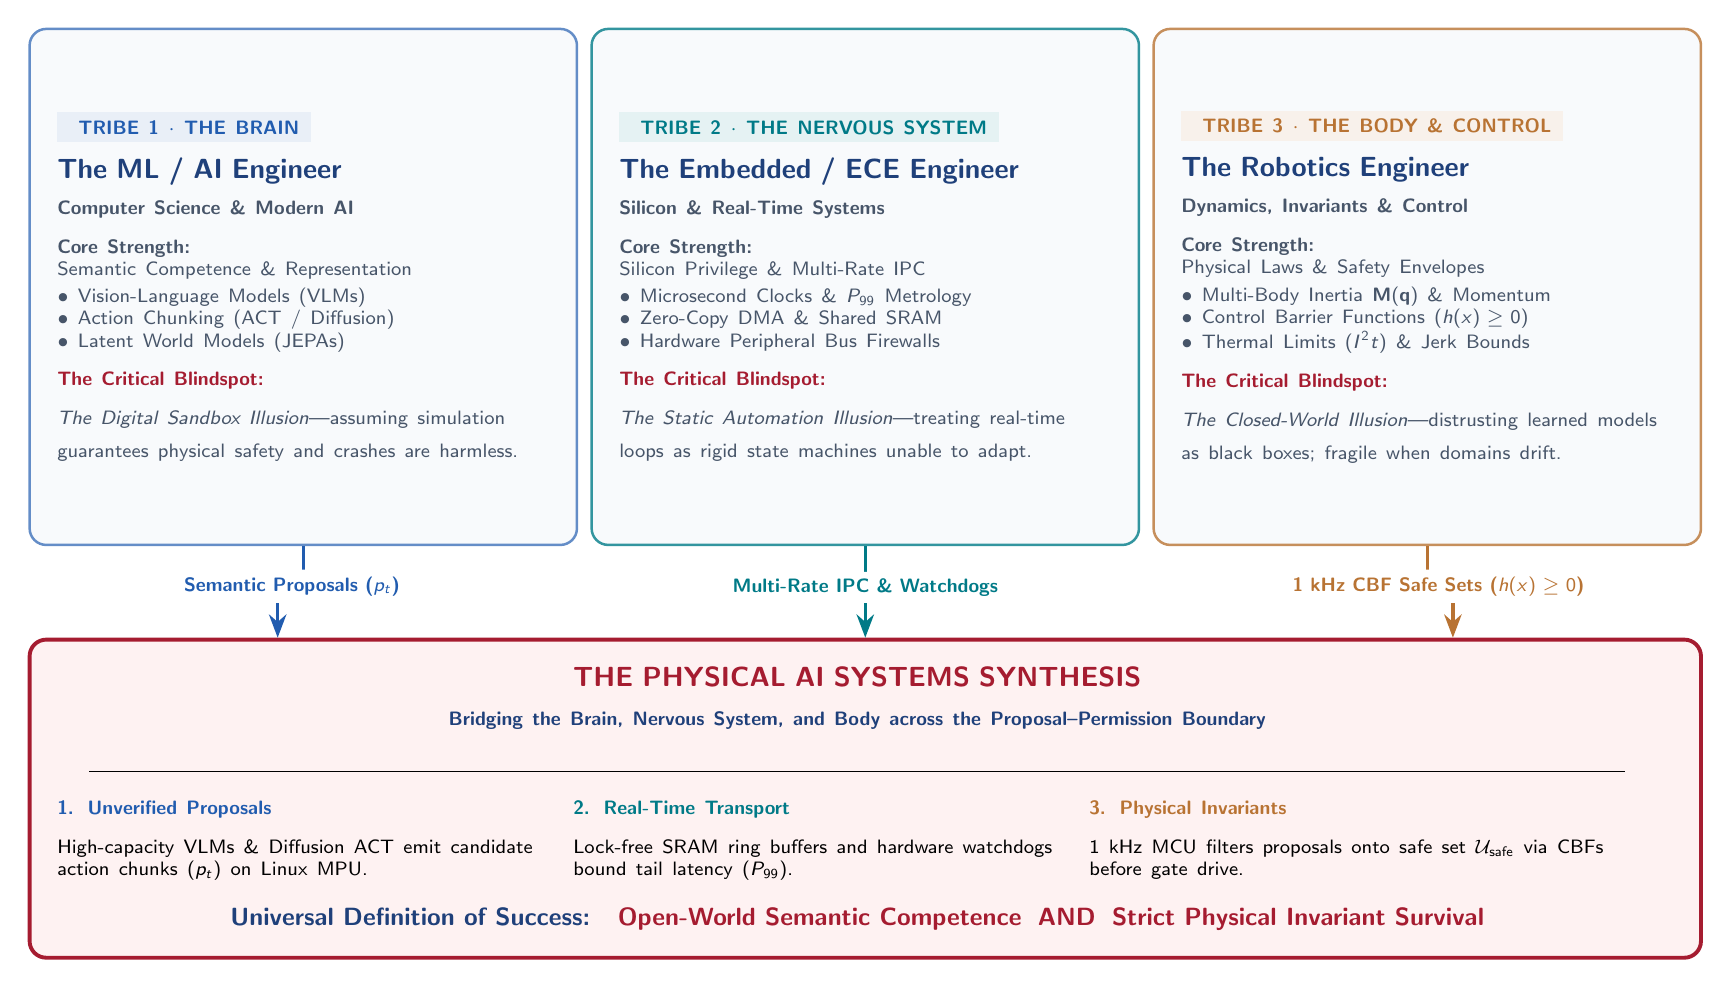
\begin{tikzpicture}[
  font=\sffamily,
  >=Stealth,
  tribecard/.style={
    draw=cardborder,
    fill=cardbg,
    rounded corners=6pt,
    line width=0.9pt,
    text width=2.46in,
    minimum height=2.58in,
    inner sep=10pt,
    align=left,
    anchor=north
  },
  synthesiscard/.style={
    draw=harvardcrimson,
    fill=frontierbg,
    rounded corners=6pt,
    line width=1.4pt,
    text width=8.08in,
    inner sep=10pt,
    align=left
  },
  arrowlabel/.style={
    font=\sffamily\scriptsize\bfseries,
    fill=white,
    inner sep=2.5pt,
    rounded corners=2pt
  }
]

  % --- TRIBE 1: The Brain (ML / AI) ---
  \node[tribecard, draw=ethblue!70] (brain) at (0,0) {
    {\scriptsize\bfseries\color{ethblue}\colorbox{ethblue!10}{\, TRIBE 1 $\cdot$ THE BRAIN\,}}\\[4pt]
    {\normalsize\bfseries\color{ethdarkblue}The ML / AI Engineer}\\[1pt]
    {\scriptsize\bfseries\color{ethslate}Computer Science \& Modern AI}\\[6pt]
    {\scriptsize\color{ethslate}\raggedright
    \textbf{Core Strength:}\\
    Semantic Competence \& Representation\\[2pt]
    $\bullet$ Vision-Language Models (VLMs)\\
    $\bullet$ Action Chunking (ACT / Diffusion)\\
    $\bullet$ Latent World Models (JEPAs)\\[6pt]
    \textbf{\color{harvardcrimson}The Critical Blindspot:}\\[2pt]
    \textit{The Digital Sandbox Illusion}---assuming simulation guarantees physical safety and crashes are harmless.
    }
  };

  % --- TRIBE 2: The Nervous System (Embedded / ECE) ---
  \node[tribecard, draw=ethpetrol!80] (nervous) at (2.81in,0) {
    {\scriptsize\bfseries\color{ethpetrol}\colorbox{ethpetrol!10}{\, TRIBE 2 $\cdot$ THE NERVOUS SYSTEM\,}}\\[4pt]
    {\normalsize\bfseries\color{ethdarkblue}The Embedded / ECE Engineer}\\[1pt]
    {\scriptsize\bfseries\color{ethslate}Silicon \& Real-Time Systems}\\[6pt]
    {\scriptsize\color{ethslate}\raggedright
    \textbf{Core Strength:}\\
    Silicon Privilege \& Multi-Rate IPC\\[2pt]
    $\bullet$ Microsecond Clocks \& $P_{99}$ Metrology\\
    $\bullet$ Zero-Copy DMA \& Shared SRAM\\
    $\bullet$ Hardware Peripheral Bus Firewalls\\[6pt]
    \textbf{\color{harvardcrimson}The Critical Blindspot:}\\[2pt]
    \textit{The Static Automation Illusion}---treating real-time loops as rigid state machines unable to adapt.
    }
  };

  % --- TRIBE 3: The Body & Control (Robotics / Mechanical) ---
  \node[tribecard, draw=ethbronze!80] (body) at (5.62in,0) {
    {\scriptsize\bfseries\color{ethbronze}\colorbox{ethbronze!10}{\, TRIBE 3 $\cdot$ THE BODY \& CONTROL\,}}\\[4pt]
    {\normalsize\bfseries\color{ethdarkblue}The Robotics Engineer}\\[1pt]
    {\scriptsize\bfseries\color{ethslate}Dynamics, Invariants \& Control}\\[6pt]
    {\scriptsize\color{ethslate}\raggedright
    \textbf{Core Strength:}\\
    Physical Laws \& Safety Envelopes\\[2pt]
    $\bullet$ Multi-Body Inertia $\mathbf{M}(\mathbf{q})$ \& Momentum\\
    $\bullet$ Control Barrier Functions ($h(x) \ge 0$)\\
    $\bullet$ Thermal Limits ($I^2t$) \& Jerk Bounds\\[6pt]
    \textbf{\color{harvardcrimson}The Critical Blindspot:}\\[2pt]
    \textit{The Closed-World Illusion}---distrusting learned models as black boxes; fragile when domains drift.
    }
  };

  % --- SYNTHESIS BANNER: Physical AI Systems ---
  \node[synthesiscard, anchor=north] (synthesis) at (2.81in, -3.05in) {
    \begin{minipage}{0.99\linewidth}
      \centering
      {\normalsize\bfseries\color{harvardcrimson} THE PHYSICAL AI SYSTEMS SYNTHESIS}\\[2pt]
      {\scriptsize\bfseries\color{ethdarkblue}Bridging the Brain, Nervous System, and Body across the Proposal--Permission Boundary}\\[5pt]
      \rule{0.96\linewidth}{0.4pt}\\[6pt]
      \begin{tabular*}{\linewidth}{@{}p{2.58in}@{\hfill}p{2.58in}@{\hfill}p{2.58in}@{}}
        \scriptsize\textbf{\color{ethblue} 1. Unverified Proposals} & 
        \scriptsize\textbf{\color{ethpetrol} 2. Real-Time Transport} & 
        \scriptsize\textbf{\color{ethbronze} 3. Physical Invariants} \\[2pt]
        \scriptsize\raggedright High-capacity VLMs \& Diffusion ACT emit candidate action chunks ($p_t$) on Linux MPU. &
        \scriptsize\raggedright Lock-free SRAM ring buffers and hardware watchdogs bound tail latency ($P_{99}$). &
        \scriptsize\raggedright 1 kHz MCU filters proposals onto safe set $\mathcal{U}_{\text{safe}}$ via CBFs before gate drive.
      \end{tabular*}\\[7pt]
      {\small\bfseries\color{ethdarkblue}Universal Definition of Success: } 
      {\small\color{harvardcrimson}\textbf{Open-World Semantic Competence} $\;\mathbf{AND}\;$ \textbf{Strict Physical Invariant Survival}}
    \end{minipage}
  };

  % Connecting Arrows from Tribes to Synthesis with Generous Clearance
  \draw[->, line width=1.2pt, draw=ethblue] (brain.south) -- ++(0,-0.20in) -| ($(synthesis.north west) + (1.25in, 0)$)
    node[pos=0.22, arrowlabel, text=ethblue] { Semantic Proposals ($p_t$)};

  \draw[->, line width=1.2pt, draw=ethpetrol] (nervous.south) -- (synthesis.north)
    node[pos=0.45, arrowlabel, text=ethpetrol] { Multi-Rate IPC \& Watchdogs};

  \draw[->, line width=1.2pt, draw=ethbronze] (body.south) -- ++(0,-0.20in) -| ($(synthesis.north east) + (-1.25in, 0)$)
    node[pos=0.22, arrowlabel, text=ethbronze] { 1 kHz CBF Safe Sets ($h(x) \ge 0$)};

\end{tikzpicture}
\end{document}
